\documentclass[tikz,border=2mm]{standalone}
\usetikzlibrary{calc,quotes,intersections, angles}
\usepackage{tkz-euclide}

\begin{document}
    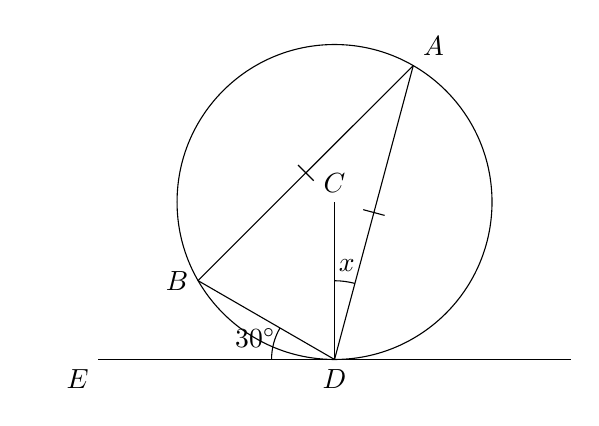
\begin{tikzpicture}[scale=2]
    % mark points on circle
        \coordinate[label = above:$C$] (C) at (0,0);
        \coordinate[label=below:$D$] (D) at (-90:1);

    % draw chords and circle
        \draw[name path=circ] (0,0) circle (1);
        \draw (C) -- (D);

    % draw tangent
        \draw (D) -- ($(D)!1.5!-90:(C)$) coordinate (L);
        \draw (D) -- ($(D)!1.5!90:(C)$) coordinate (E);

    % 
        \path[name path=DB] (D) -- ($(D)!1.5!-30:(E)$);
        \path[name path=DA] (D) -- ($(D)!2!-15:(C)$);
        \path[name intersections={of=DB and circ, by={B}}];
        \path[name intersections={of=DA and circ, by={A,temp}}];

    \draw (D) -- (B);
    \draw (A) -- (D);
    \draw (A) -- (B);

    % Label points E and B
    \node at (E) [anchor=north east] {$E$};
    \node at (B) [anchor= east] {$B$};
    \node at (A) [anchor = south west] {$A$};

    % \draw (C) -- (B);
    % % \draw (A) -- (D);
    \tkzMarkSegment[pos=.5,mark=|](A,B);
    \tkzMarkSegment[pos=.5,mark=|](A,D);
    
    \pic [draw, "$30^\circ$", angle eccentricity=1.3, angle radius = 0.8cm] {angle = B--D--E};
    \pic [draw, "$x$", angle eccentricity=1.2, angle radius = 1cm] {angle = A--D--C};
        
    \end{tikzpicture}
\end{document}